\chapter{绪论}

\section{研究背景与意义}


毫米波雷达作为一种先进的感知技术,在自动驾驶、无人机导航、智能交通系统和工业自动化等领域获得了广泛关注。它具有高分辨率、强穿透能力和良好的环境适应性,即使在雨雪、雾霾等恶劣天气条件下也能稳定工作。《新能源汽车产业发展规划(2021—2035年)》\cite{xbngyrqiie2020}指出,到2025年,新能源汽车新车销售量将达到汽车新车销售总量的20\%左右,自动驾驶的安全水平将全面提升,车载毫米波雷达和激光雷达将成为L2及以上自动驾驶的标配。

激光雷达由于其工作原理,性能常受光照变化和恶劣天气影响。相比之下,毫米波雷达在光照变化、烟雾、雾霾等能见度低的条件下依然能有效工作。尽管毫米波雷达生成的点云数据较为稀疏且噪声较高,但在这些条件下依然能够感知外部环境\cite{qian20203d},成为自动驾驶和环境监测中的重要技术。

点云是一种数据表示形式,主要用于3D建模或测量领域,每个点在空间中表示一个具体的位置。使用点云数据描述物体的方式广泛应用于捕捉和表现物理世界中的各种形状和场景。

点云配准是将多个点云数据集整合到一个统一的坐标系统中的过程。例如,在自动驾驶领域,通过点云配准,车辆能够更准确地识别和定位周围的物体和环境特征,实现更安全的导航。在环境建模方面,通过配准不同视角和位置的点云数据,可以创建出精确的三维模型用于进一步的分析和可视化处理。到目前为止,学术界和工业界已有大量适用于非毫米波雷达的配准方案。

由于毫米波雷达能在激光雷达无法工作的情况下保持正常运作,研究适合毫米波雷达点云数据的检测与配准方案变得尤为重要。在毫米波雷达点云配准中,存在两个待解决的主要问题。首先,由于毫米波雷达的工作频率较低,通常会产生较高水平的噪声。在低信噪比、多目标的情况下,使用恒虚警率(Constant False Alarm Rate,CFAR)算法\cite{7185}生成毫米波雷达点云中的目标点时,存在性能退化和无法有效提取目标点的问题。因此,如何在噪声环境中准确地识别和检测出目标点面临严峻挑战。
其次,毫米波雷达获取的点云数据往往比较稀疏,并且点的密度不均匀。而稀疏以及不均匀性可能导致适用于激光雷达的传统配准方案在毫米波雷达点云配准过程中出现位置偏差或配准不精确的问题,进而影响到自动驾驶、环境监测等应用的性能和可靠性。因此,需针对噪声干扰和点云稀疏性的研究有效配准算法,以确保毫米波雷达点云数据能够准确地在不同坐标系下进行配准和使用。

\section{研究面临的问题}
毫米波雷达点云不同于激光雷达点云,由于其工作频率较低、受噪声干扰较大,导致难以检测出有效目标点数据,且目标点形成的点云数据具有稀疏、密度不均匀的特点。

\textbf{问题一:存在未知的噪声干扰,难以有效检测目标点}
\par
在毫米波雷达工作时,收到的回波信号除了有效目标点的信息,还包括路边建筑的反射、目标的多次反射、多径效应等带来的噪声\cite{richards2010principles}。噪声的干扰导致在提取毫米波雷达点云的有效目标点时会产生虚假点云。由于传统的CFAR算法在处理毫米波雷达回波信号时,只能关注有限的训练单元,导致CFAR算法在判断距离多普勒图中是否有目标存在时,只能考虑到特定的局部信息,而无法全面考虑整个场景的复杂情况,在低信噪比、多目标的情况下,会因为虚假点云而导致检测目标点的性能下降。
\par
\textbf{问题二:毫米波雷达点云密度稀疏且不均匀,传统配准算法难以工作}
\par
点云配准算法,如迭代最近点(Iterative Closest Point,ICP)算法\cite{besl1992method}等对于待配准点云要求有明显可识别的特征,这些特征在配准过程中用于识别对应的点,此外配准的效果依赖点云中点的数量,需要大量的点信息提高配准效果。毫米波雷达在工作时使用扫描的方式,在靠近雷达处扫描到的点云较为稠密而远离雷达处的点云较为稀疏,使得在多个不同位置工作的毫米波雷达对于统一物体扫描所得到的点云稀疏程度不一致,导致对于同一物体特征的识别变得困难。毫米波雷达工作频率较低、波长较长的特征使毫米波雷达拥有了更强的穿透力和检测距离,但是这也导致了范围分辨率较低。60GHz的毫米波雷达距离分辨率约为3.75cm\cite{meta2007signal},而激光雷达的分辨率可以达到毫米级,毫米波的原理决定了其点云无法达到激光雷达的分辨率。点云密度不均匀和点云密度稀疏的问题导致传统配准算法难以工作。
\section{国内外研究现状}
在上述研究背景下,本节对毫米波雷达回波信号目标点检测方案和毫米波雷达点云配准方案当前的国内外研究现状进行了总结和分析。
\subsection{毫米波雷达目标点检测}
目前雷达回波信号目标点检测算法主要分为两大类,基于检测单元平均值统计评估的CFAR算法以及CFAR算法的改进和基于深度学习的点云目标点检测。

\par
(1)传统目标点检测方法
\par
传统的雷达回波信号目标检测大多是基于CAFR算法的改进,此类算法主要方法是根据参考单元杂波噪声识别进行评估得到平均背景噪声水平,根据虚警率计算阈值因子,使用阈值因子与平均背景噪声水平相乘以得到检测阈值的恒定虚警率检测算法。最早的CFAR算法是单元平均恒虚警率算法(Cell Average CFAR,CA-CFAR)\cite{4043676},CA-CFAR利用周围参考单元的平均值作为噪声水平的评估。然而,CA-CFAR在多目标以及非均匀噪声的环境下检测效性能会急剧下降。对CA-CFAR改进的算法有最大平均恒虚警率算法( Greatest of CFAR,GO-CFAR)\cite{4102285}和最小平均恒虚警率算法(Smallest of CFAR,SO-CFAR)\cite{trunk1978range}。GO-CFAR可以良好地控制虚警率但是在多目标情况下无法正确评估噪声水平。SO-CFAR在多目标环境的目标点检测有良好的效果,但是无法良好地控制虚警率。为改进基于平均值的CFAR在多目标场景下的检测性能下降,Rohling提出了基于有序统计的CFAR检测算法( Ordered Statistic CFAR,OS-CFAR)\cite{4102829},通过将排序后的第k个值作为背景噪声水平估计值计算检测阈值。但是OS-CFAR的k值选择会极大的影响检测性能。Wang等人提出了一种新的密度审查操作\cite{WangCFAR},在局部 CFAR 检测之前快速识别去除大量无信息背景杂波,减少了后续CFAR检测的计算成本以及由此产生的误报数量。但是这些方法都无法有效解决多目标时目标点误报问题。

\par
(2)基于深度学习的目标点检测方法
\par
基于深度学习目标检测技术,依托于神经网络对特征的提取和抽象能力,为毫米波雷达的目标点检测提供了新的思路\cite{mata2015mlp}。
Akhtar等人以OS-CFAR为基础,提出了使用多层MLP神经网络辅助OS-CFAR设置动态阈值的方案\cite{akhtar2021training}。
Kang等人提出了基于Faster R-CNN的检测方案\cite{R-CNN-CFAR},该方案使用Faster R-CNN生成CFAR算法的保护单元,优化了小目标检测性能。Lin等人提出了基于卷积神经网络的CFAR方案\cite{DL-CFAR},降低了多目标场景中掩蔽效应的影响,在信噪比的情况下表现良好。
Faruk等人提出了基于CNN\cite{lecun1989backpropagation}的毫米波雷达目标点检测RadCNN\cite{CNN-CFAR},该方案使用分块输入距离多普勒图到CNN的方式返回预测后的分块结果。
Cao等人提出了基于DNN\cite{DBLP:conf/nips/KrizhevskySH12}的毫米波雷达峰值检测方案\cite{DNN-CFAR},该方案将目标点检测问题转化为频率强度序列分类问题。
Cheng等人提出了避免虚假点的新方案\cite{9823311},设计了一个编码器-解码器的网络,使用的标签为LiDAR检测数据。编码器的输入为距离多普勒图,解码器的输出为一个预测标签的矩阵,表示在距离多普勒图上的每个单元是否为目标点。但是该方案需要使用LiDAR配套生成训练数据,且LiDAR数据没有多普勒维度,用于对距离多普勒图做预测的效果不佳。
Zhao等人,提出了使用DBSCAN\cite{schubert2017dbscan}结合ANN网络\cite{agatonovic2000basic}的方案,使用DBSCAN聚类排除目标附近因为旁瓣效应带来的干扰峰值,使用ANN估计背景噪声的参数\cite{sym11121482}。但是该方案因为引入了DBSCAN导致计算需要花费更多的时间,并且在低信噪比的情况下性能会降低。
Akarsh的方案RadarHD\cite{10161429}与上面的方案不同,不再使用传统的快速傅里叶变化(Fast Fourier Transform,FFT)处理后的距离多普勒图来检测有效目标点,而是设计了一个端到端的神经网络,使用雷达原始的I/Q数据作为输入,使用激光雷达对同一片环境的稠密点云作为标签训练了点云生成网络。该方案虽然能够生成高质量点云,但是需要激光雷达的数据作为标定,适用性不强。
\subsection{毫米波雷达点云配准}

\par
(1)传统点云配准
\par
传统的点云配准方案如迭代最近点、核心相关(Kernel Correlation,KC)\cite{DBLP:journals/cad/SongHDLY22}、鲁棒点匹配(Robust Point Matching,RPM)\cite{ma2014robust}等,通过匹配源点云和参考点云的特征点,迭代计算出最优的配准变换矩阵以最小化点云之间的距离。ICP算法通过迭代优化对应点对之间的距离,实现点云的配准;RPM算法通过计算源点云和参考点云中点与点的对应关系,找到对应点对后进行配准;KC算法通过寻找待配准点云之间的相似性,找出最大相似性后计算出最优的变换矩阵以实现配准。然而,这些传统算法都在处理毫米波雷达点云时面临困难,因为毫米波雷达点云通常稀疏且易受噪声影响,使得传统算法的性能下降。

\par
(2)基于深度学习的点云配准
\par
检测到毫米波雷达目标点后,需要将多个雷达的目标点数据配准到同一个坐标系的点云下。由于毫米波雷达点云密度稀疏且不均匀的特性,许多专家学者在其点云的配准上进行了大量的研究。
Shastri等人提出了mmSCALE\cite{mmSCALE},通过利用环境中人员的运动轨迹自动估计多个雷达相对于参考坐标系的位置和方向,使用奇异值分解(Singular Value Decomposition,SVD)最小二乘法(Least Sqaure Method,LS)获取毫米波雷达的相对位置和方向。但是此方案所适用场景为毫米波雷达部署之前,预先估计出坐标变化,不适用于已有点云数据的配准。
Chen等人\cite{9827800}提出了通过标记的方式配准点云。通过预先设置标记点并构建其点云数据,自动泊车系统能够在运行过程中利用多帧融合技术准确捕获这些标记点的特征,借助标记点特征完成配准。此方案精度较高但是在无法安装标记点的场景无法使用。
Yeong等人提出了在低能见度的情况下,使用毫米波雷达生成点云的方案\cite{8967633}。其方案使用预先构建的密集 LiDAR 点云辅助毫米波雷达雷达测量结果以进行定位,在激光雷达无法工作的环境使用毫米波雷达点云数据依据预先构建的激光雷达图,通过点云配准感知如浓雾等环境中的情况。但是该方案依赖于使用激光雷达先进行地形图的扫描,使用比较局限。Yew等人提出了使用PointNet\cite{qi2017pointnet}提取点云特征的方案\cite{Yew_2020_CVPR},Xiang等人提出了使用DBSCAN\cite{DBLP:conf/kdd/EsterKSX96}进行空间聚类进行特征提取的方案\cite{DBLP:journals/iotj/XiangMTYWGCKY24},这两个方案提高了提取单个点特征的丰富程度,但是无法克服点云密度不均匀带来的特征在密度不同处不适用的问题。
\section{论文研究内容与主要工作}
在毫米波雷达工作过程中,存在低信噪比、多目标的情况下难以从距离多普勒图中检测出目标点,检测出的目标点较为稀疏且分布不均匀,导致点云难以配准的问题。本文分析了现有的毫米波雷达目标点检测方案以及现有点云配准方案,结合毫米波雷达工作特点对如何有效检测目标点、如何对检测出的目标点进行有效配准做了深入研究,本文的研究内容如下:
\par
\textbf{研究内容一}:针对在低信噪比、多目标的情况下难以从距离多普勒图中提取出检测点的问题,提出一种基于残差神经网络\cite{he2016deep}和自注意力机制\cite{vaswani2017attention}的距离多普勒图处理方案RA-CFAR(Residual Attention CFAR)。RA-CFAR使用残差神经网络作为距离多普勒图局部的特征提取模块,并且通过自注意力模块结合距离多普勒图局部的空间特征自估计目标点所在单元的检测阈值。距离多普勒图是调频连续波雷达用于检测目标速度和位置的重要手段,距离多普勒的两个维度分别为速度维FFT和距离维FFT,目标的速度和距离会在距离多普勒图上呈现尖峰的形式。为了有效提取出尖峰所在单元,许多研究人员采取众多方式,如使用训练单元平均值估计CA-CFAR、训练单元排序第k大值估计OS-CFAR、采用深度学习估计训练单元的方案等。为了解决距离多普勒图检测目标点位置时,尤其是多运动目标时难以设置CFAR的参数,导致无法有效检测到目标点的问题,RA-CFAR 使用自注意力模块结合距离多普勒图局部的空间特征提出自估计阈值检测目标点所在单元的方案。并且通过与四种常用算法对比,证明RA-CFAR在处理多目标和低信噪比距离多普勒图时具有良好的性能。
\par
\textbf{研究内容二}:针对检测出的目标点较为稀疏和分布不均匀,导致点云难以配准的问题,研究当前毫米波雷达配准的主流方案,包括使用SLAM的雷达轨迹定位配准方案\cite{grisetti2010tutorial}以及点云的经典配准算法。使用SLAM的方案需要引入复杂的SLAM算法进行姿态估计并且不适用于历史点云数据的配准。经典配准算法如ICP算法,RPM算法,CPD算法\cite{cpd}等面对毫米波雷达低分辨率、稀疏且不均匀的点云配准效果不佳。分析毫米波雷达点云的特点,在点级别提出结合点云邻域的多普勒特征以及多尺度邻域的点特征提取方案即点云邻域特征提取网络。为了在点级别挖掘出更多特征,在点局部拟合法平面计算出点的法向量作为特征信息的一部分,使用点云邻域特征提取网络提取多个半径的邻域特征进行融合作为目标点最终特征。为加快配准的收敛,提出全局配准参数预测网络,使用源点云与参考点云的全局特征推测初始配准参数。迭代配准中使用源点云与参考点云的特征距离代替空间距离,使用推测的配准参数进行迭代配准。通过实验验证在毫米波雷达的点云配准中多尺度邻域特征以及配准参数推测的有效性。

\section{论文结构安排}
本论文主要分为六个章节,文章结构如图\ref{fig:论文结构安排}所示,相关内容安排如下:
\par
第一章,绪论。本章分析了毫米波雷达点云配准的研究背景和意义,分析了毫米波雷达点云配准面临的问题,总结了国内外研究现状,提出了本文的研究内容与主要工作。
\par
第二章,相关理论技术研究。本章分三个部分分别介绍了毫米波雷达相关的知识,点云配准相关的知识,深度学习相关的知识。在毫米波雷达相关知识中介绍了调频连续波雷达的工作原理,距离多普勒图的特点,以及雷达回波信号的处理。在点云配准相关知识中介绍了点云配准的基本概念,点云配准的基本流程,以及点云配准的常用算法。在深度学习相关知识中介绍了深度学习的基本概念,残差神经网络的基本结构,自注意力机制的基本原理。为后续的研究工作提供了理论基础。
\par
第三章,基于距离多普勒图空间相关性的目标点检测方案。本章首先分析了距离多普勒图的特点,研究了传统CFAR算法在处理距离多普勒图时的局限性,通过分析距离多普勒图中目标点区域的特征,提出了基于残差神经网络和自注意力机制的距离多普勒图处理方案。最后通过实验验证了RA-CFAR在处理多目标和低信噪比距离多普勒图时具有良好的性能。
\par
第四章,基于多尺度邻域的毫米波点云配准方案。本章针对毫米波雷达点云配准的问题,结合毫米波雷达点云的低分辨率、稀疏、密度分布不均匀的特点分析了传统配准算法不适用与毫米波雷达点云的原因,提出了结合点云邻域多普勒特征以及多尺度邻域特征融合的点特征提取方案即点云邻域特征提取网络,和使用源点云与参考点云的全局特征推测初始配准参数的方案即全局配准参数预测网络。经过实验验证了在毫米波雷达的点云配准中多尺度邻域特征以及配准参数推测的有效性。
\par
第五章,原型系统的设计与实现。本章将介绍毫米波雷达点云提取优化方案和点云迭代优化配准方案的具体实现,包括系统的整体架构设计、系统的模块划分、系统的具体实现细节、系统的性能测试等。验证了本文提出的方案在实际场景中的有效性。
\par
第六章,总结与展望。总结本文的研究工作,并对未来的工作进行了展望。
\begin{figure}[htbp]
	\centering
	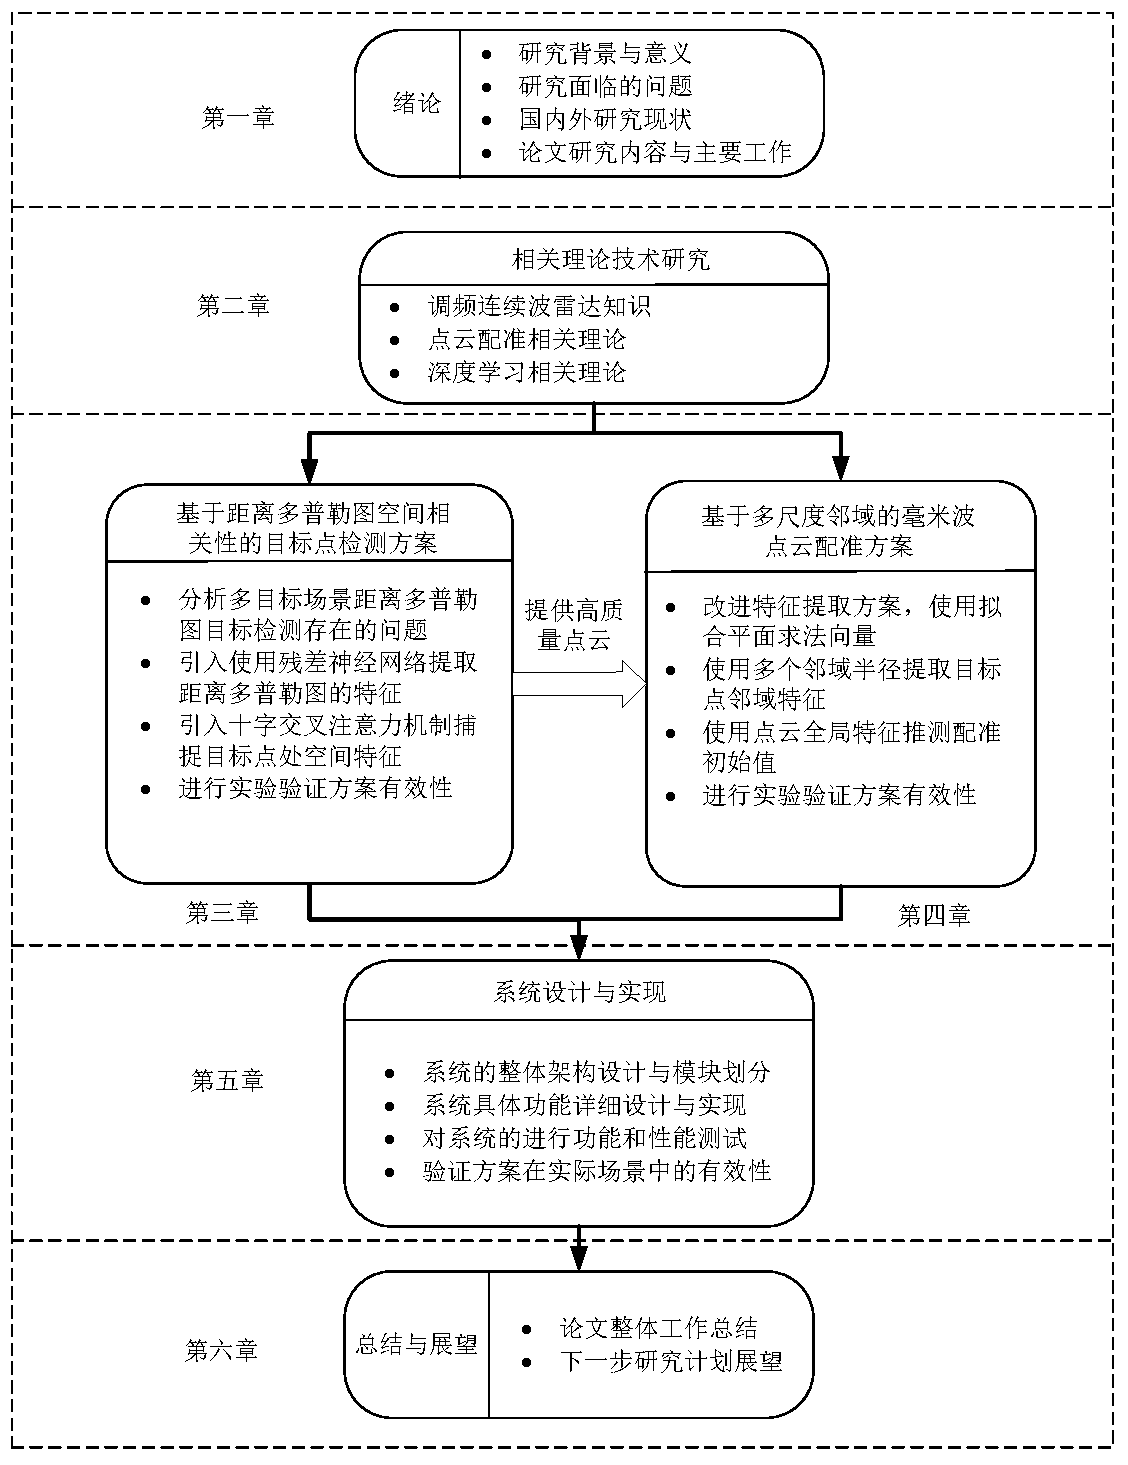
\includegraphics[width=0.95\linewidth]{figures/论文结构.pdf}
	\caption{论文结构安排}
	\label{fig:论文结构安排}
\end{figure}